\pdfminorversion=7
\documentclass[11pt]{article}
\usepackage[T1]{fontenc}
\usepackage[utf8]{inputenc}
\usepackage{lmodern}
\usepackage[margin=1in]{geometry}
\usepackage{graphicx}
\usepackage{placeins}
\usepackage{xurl}
\usepackage[colorlinks=true,linkcolor=blue,citecolor=blue,urlcolor=blue]{hyperref}
\setlength{\emergencystretch}{3em}
\title{Supplementary material\\[0.3em]
\large Rho: A Purpose-Driven Workspace for Human--AI Collaborative Analysis}
\author{Yonghe Xia \quad Guangchuang Yu}
\date{}
\begin{document}
\maketitle

\noindent This supplement holds the full interface captures behind the manuscript's five analyses. Each is a screenshot of one recorded state under one configuration (Rho 0.5.2, one agent, one model, one local machine, managed execution unavailable). A capture shows what the interface displayed; it does not by itself establish that an analysis was correct, that a displayed relationship is scientifically valid, or that a person understood or endorsed an output. Regions are rearranged or cropped for legibility; pixel content is unchanged.

\section*{Supplementary Figures}

\begin{figure}[!htbp]\centering
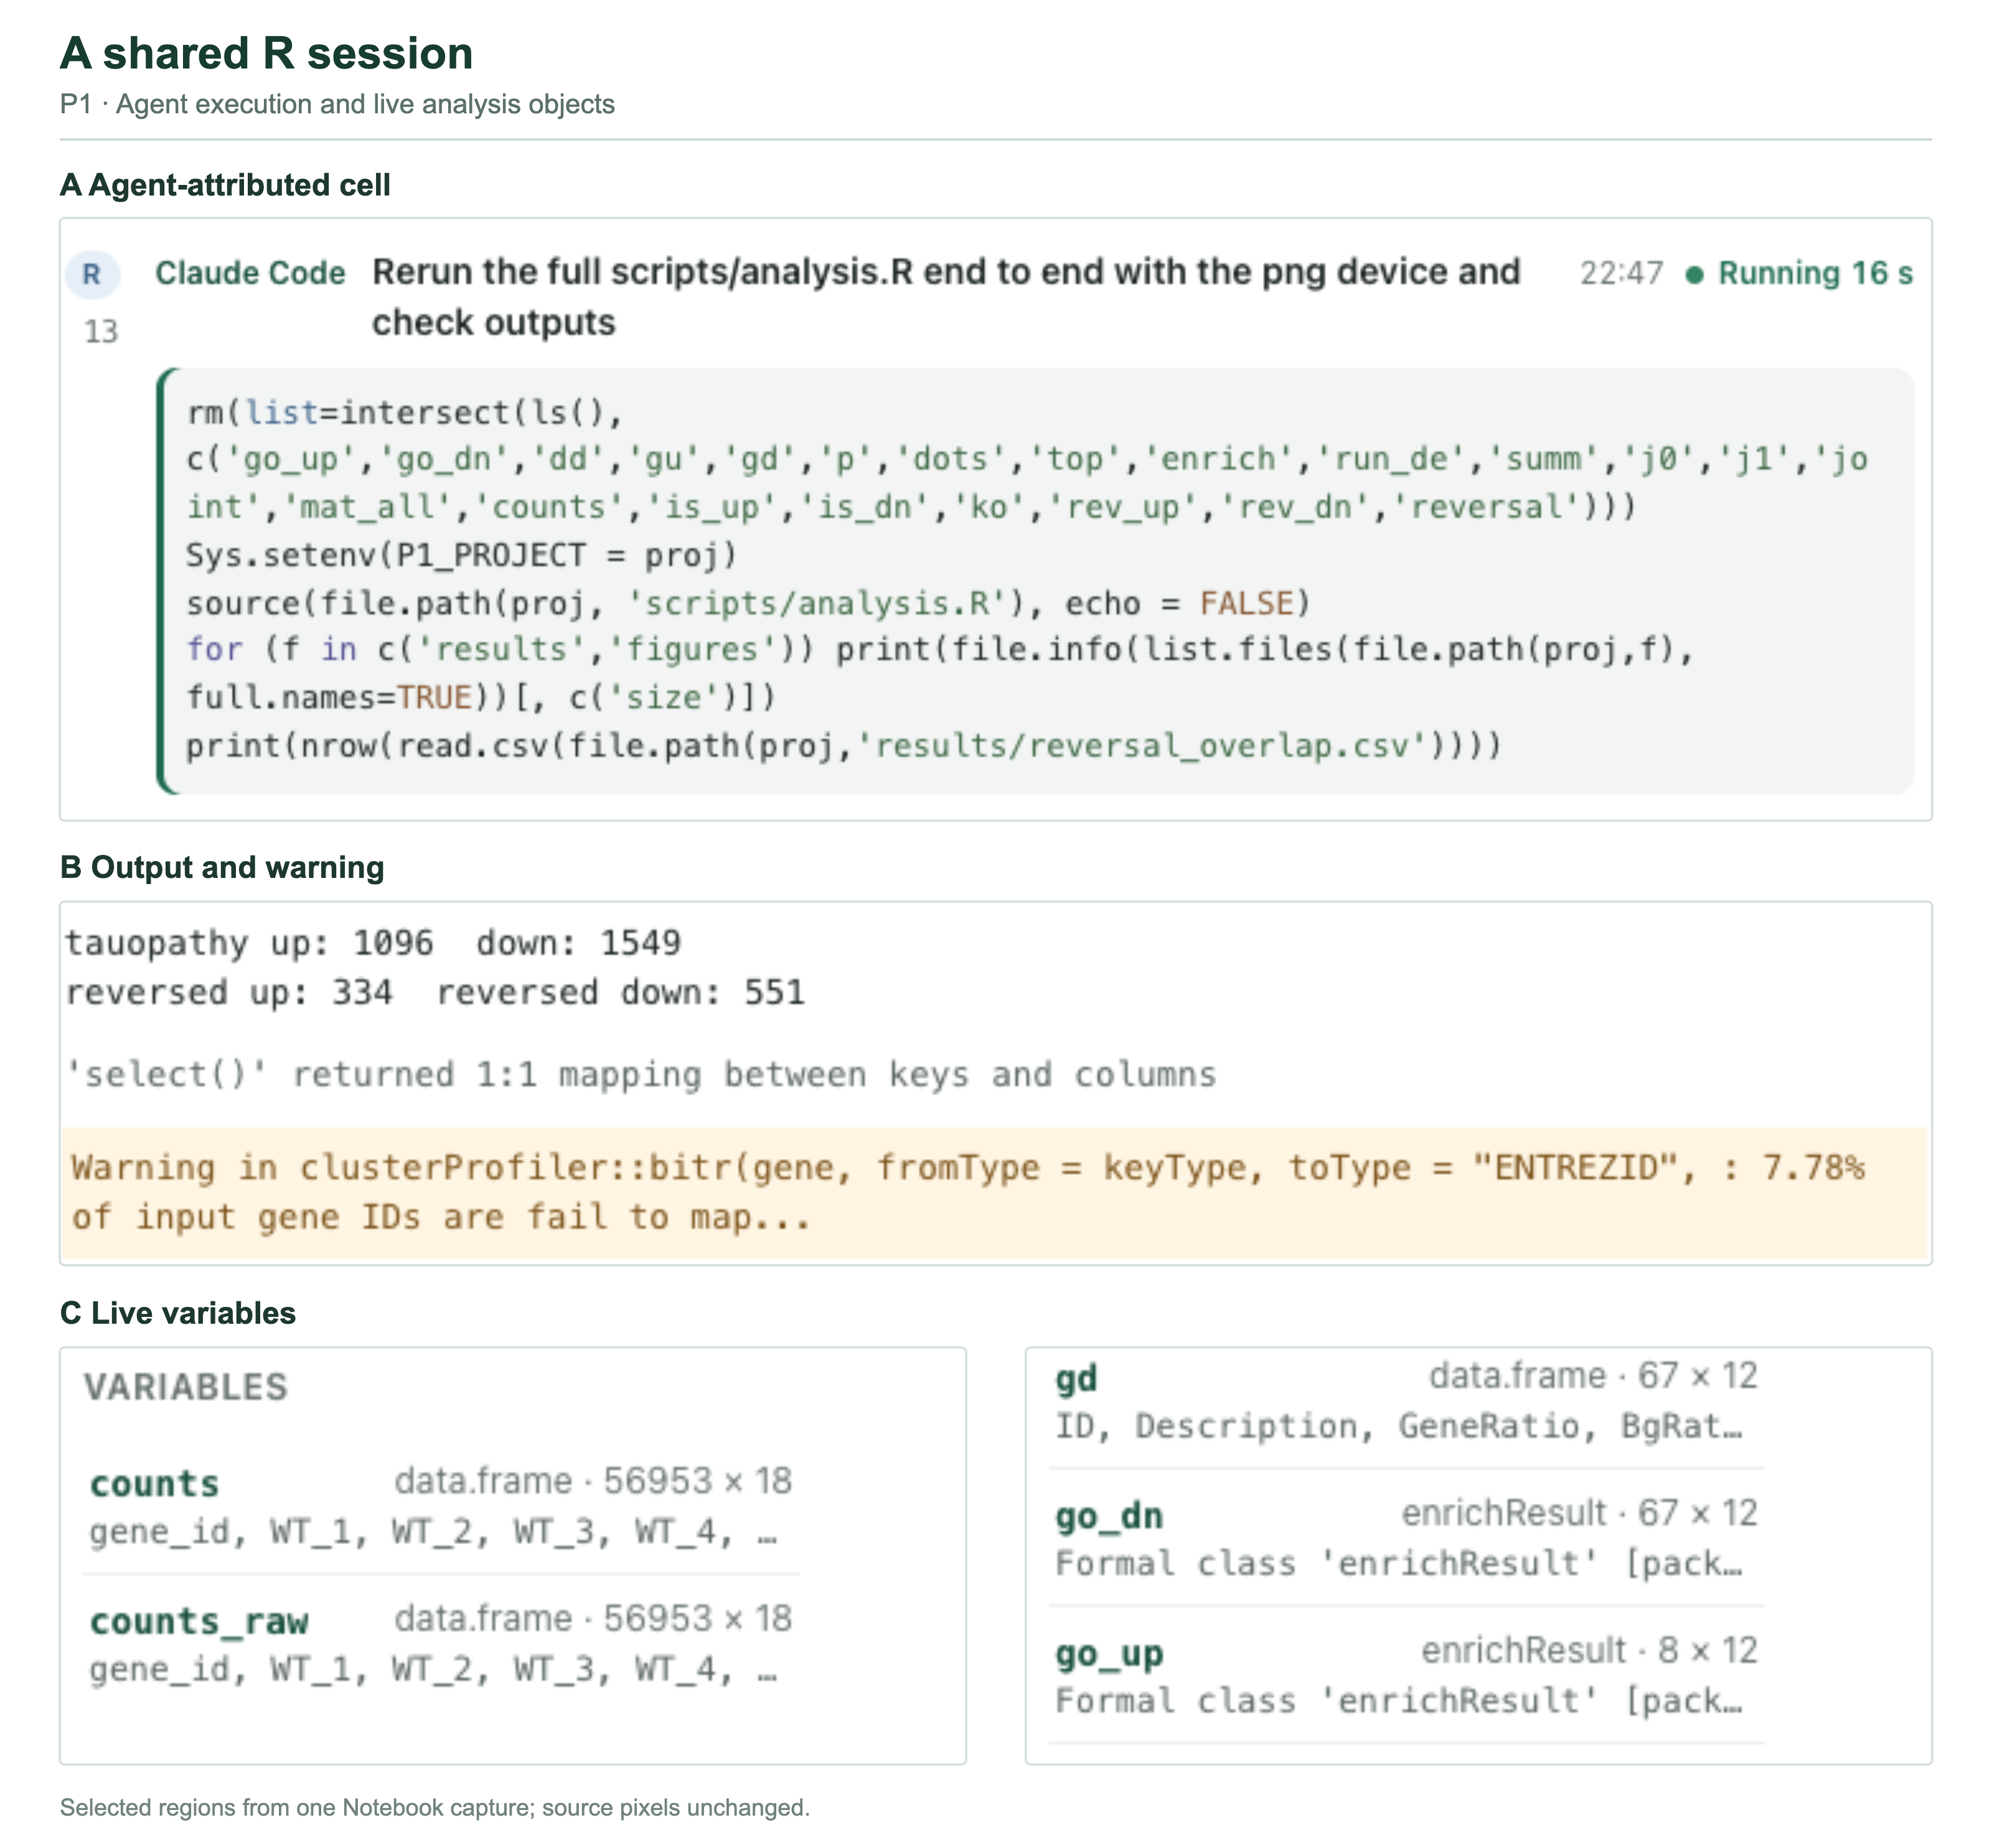
\includegraphics[width=\linewidth,height=0.9\textheight,keepaspectratio]{figures/figure-1-notebook.png}
\caption{\textbf{Figure S1. The P1 Notebook (full capture).} (A) An R cell attributed to Claude Code, with its stated purpose and elapsed time; (B) reported counts and a gene-mapping warning; (C) two parts of the live Variables pane, including \texttt{enrichResult} objects. Regions rearranged for legibility.}\end{figure}

\begin{figure}[!htbp]\centering
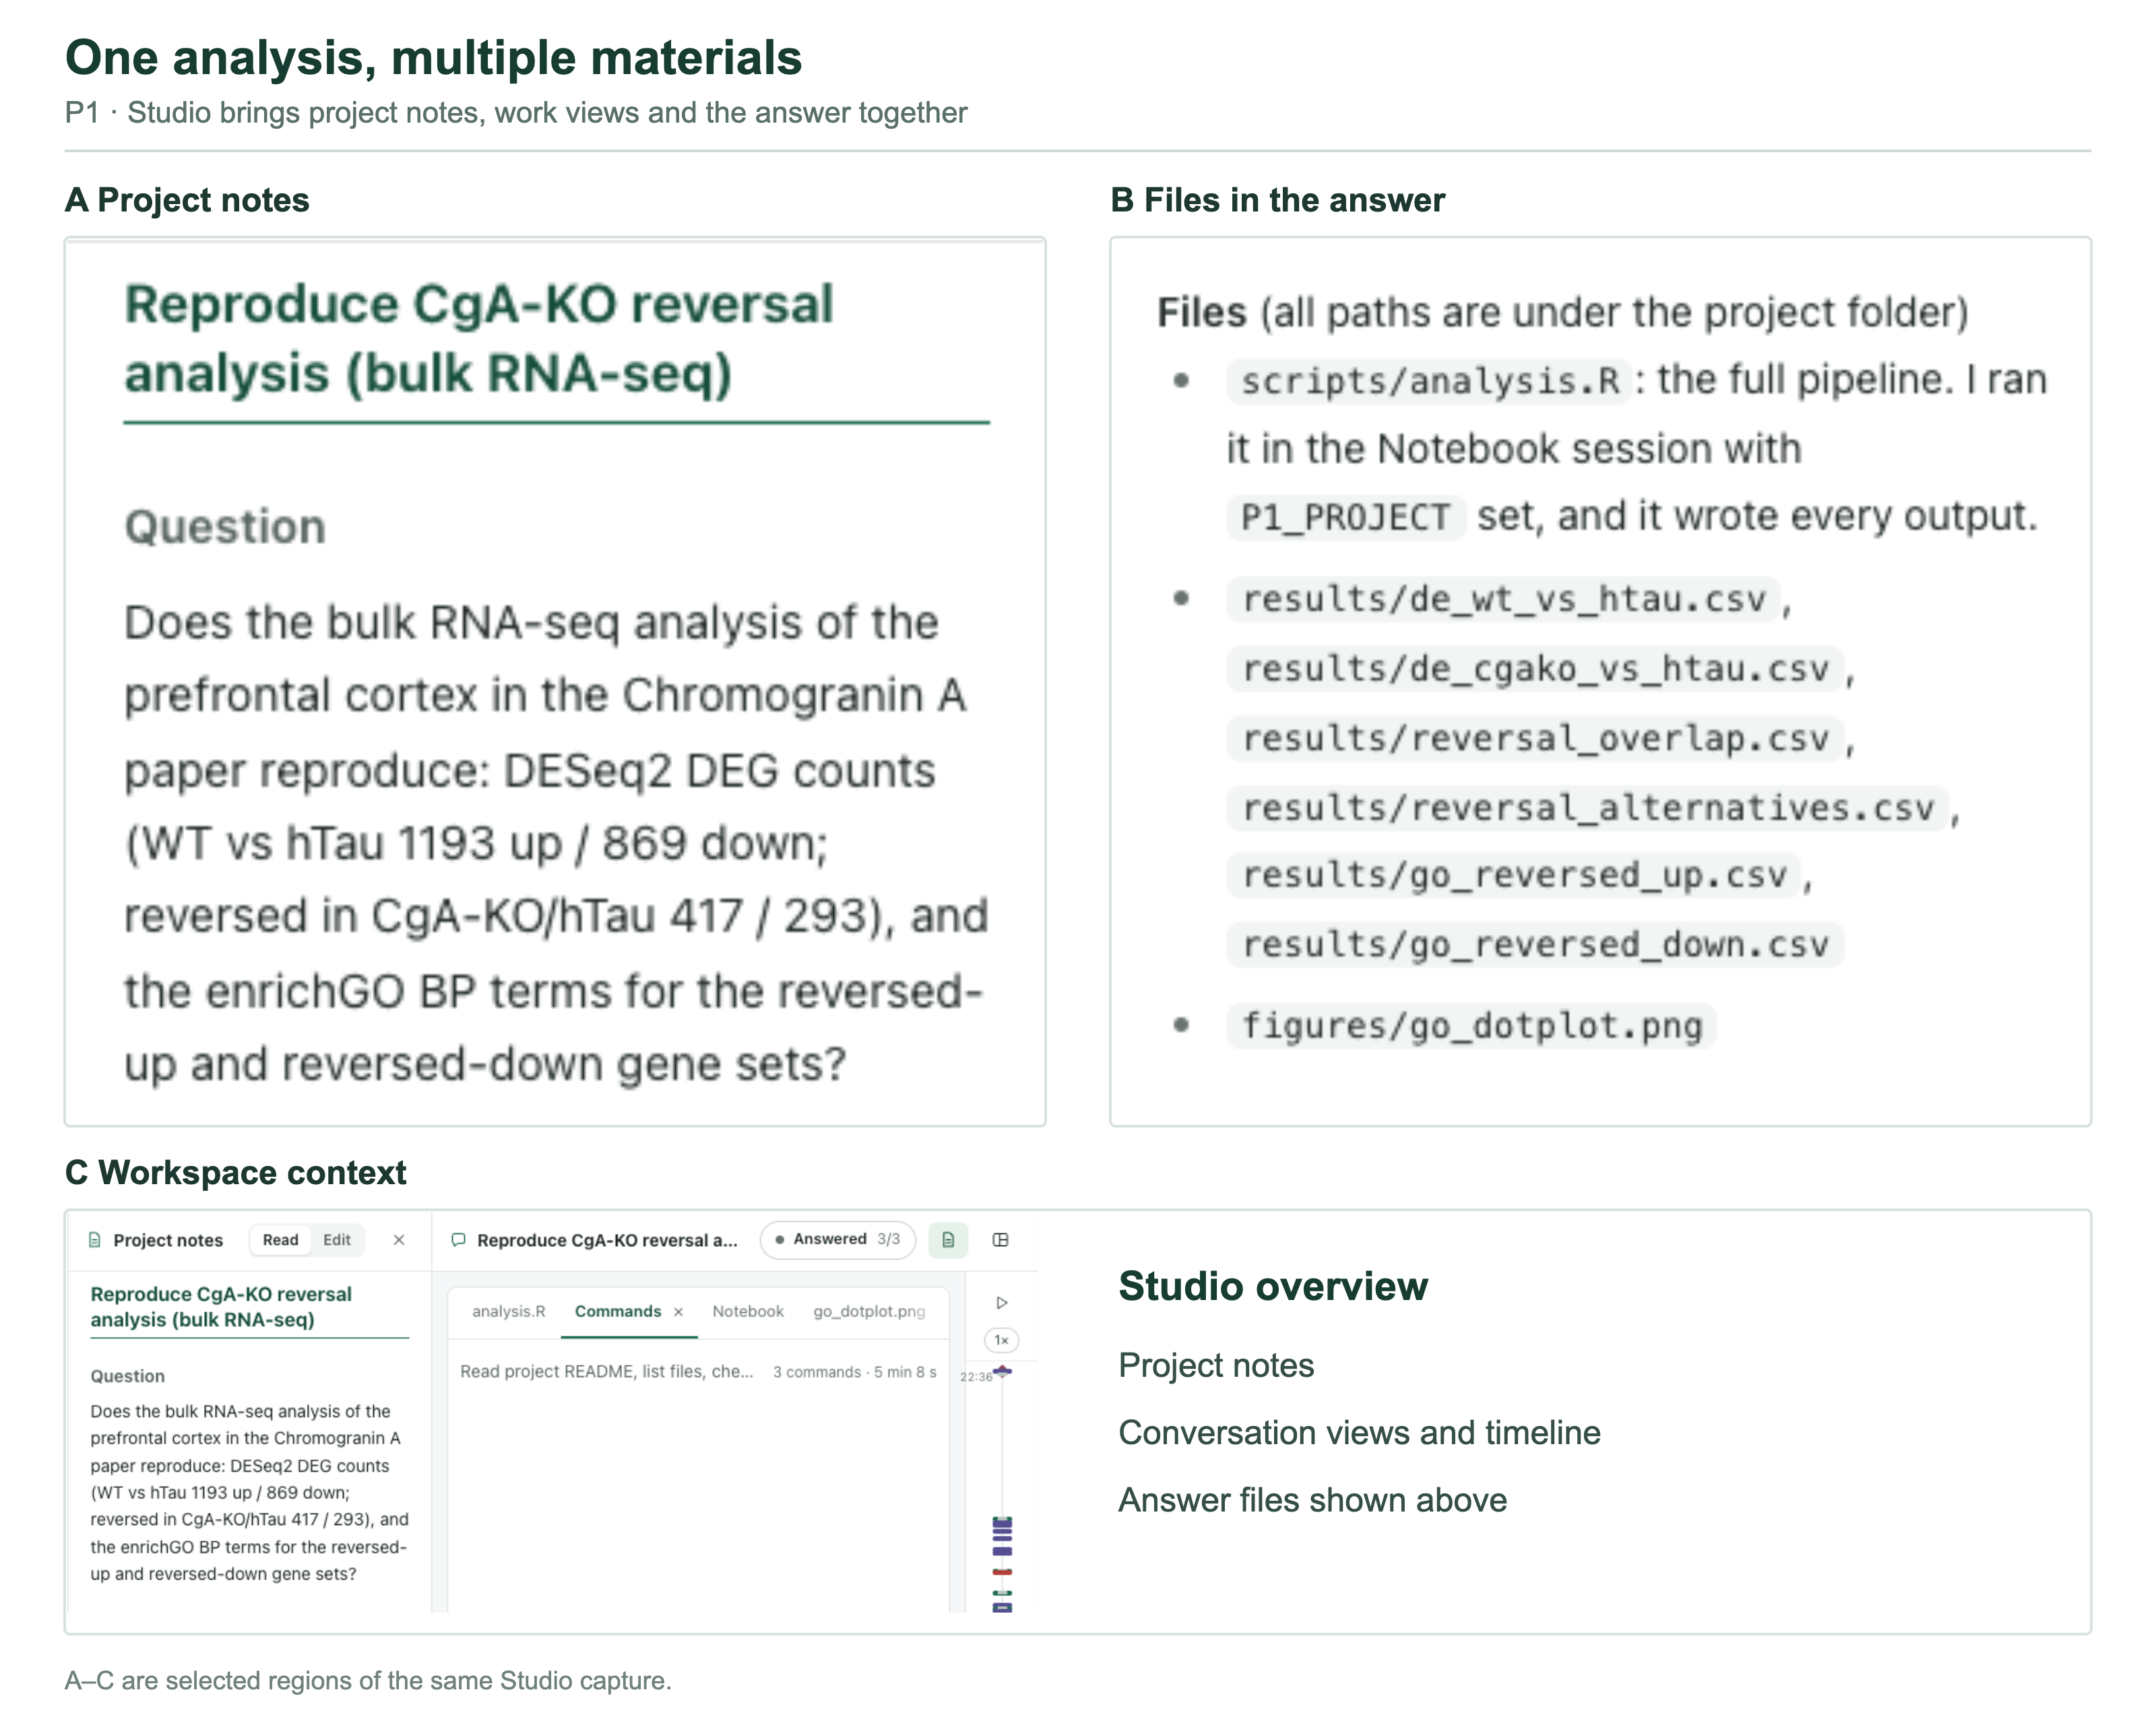
\includegraphics[width=\linewidth,height=0.9\textheight,keepaspectratio]{figures/figure-2-studio.png}
\caption{\textbf{Figure S2. P1 in Studio.} (A) The question in project notes; (B) files listed in the agent's answer; (C) the conversation's work views and timeline. Presence of a component does not establish that the agent read it.}\end{figure}

\begin{figure}[!htbp]\centering
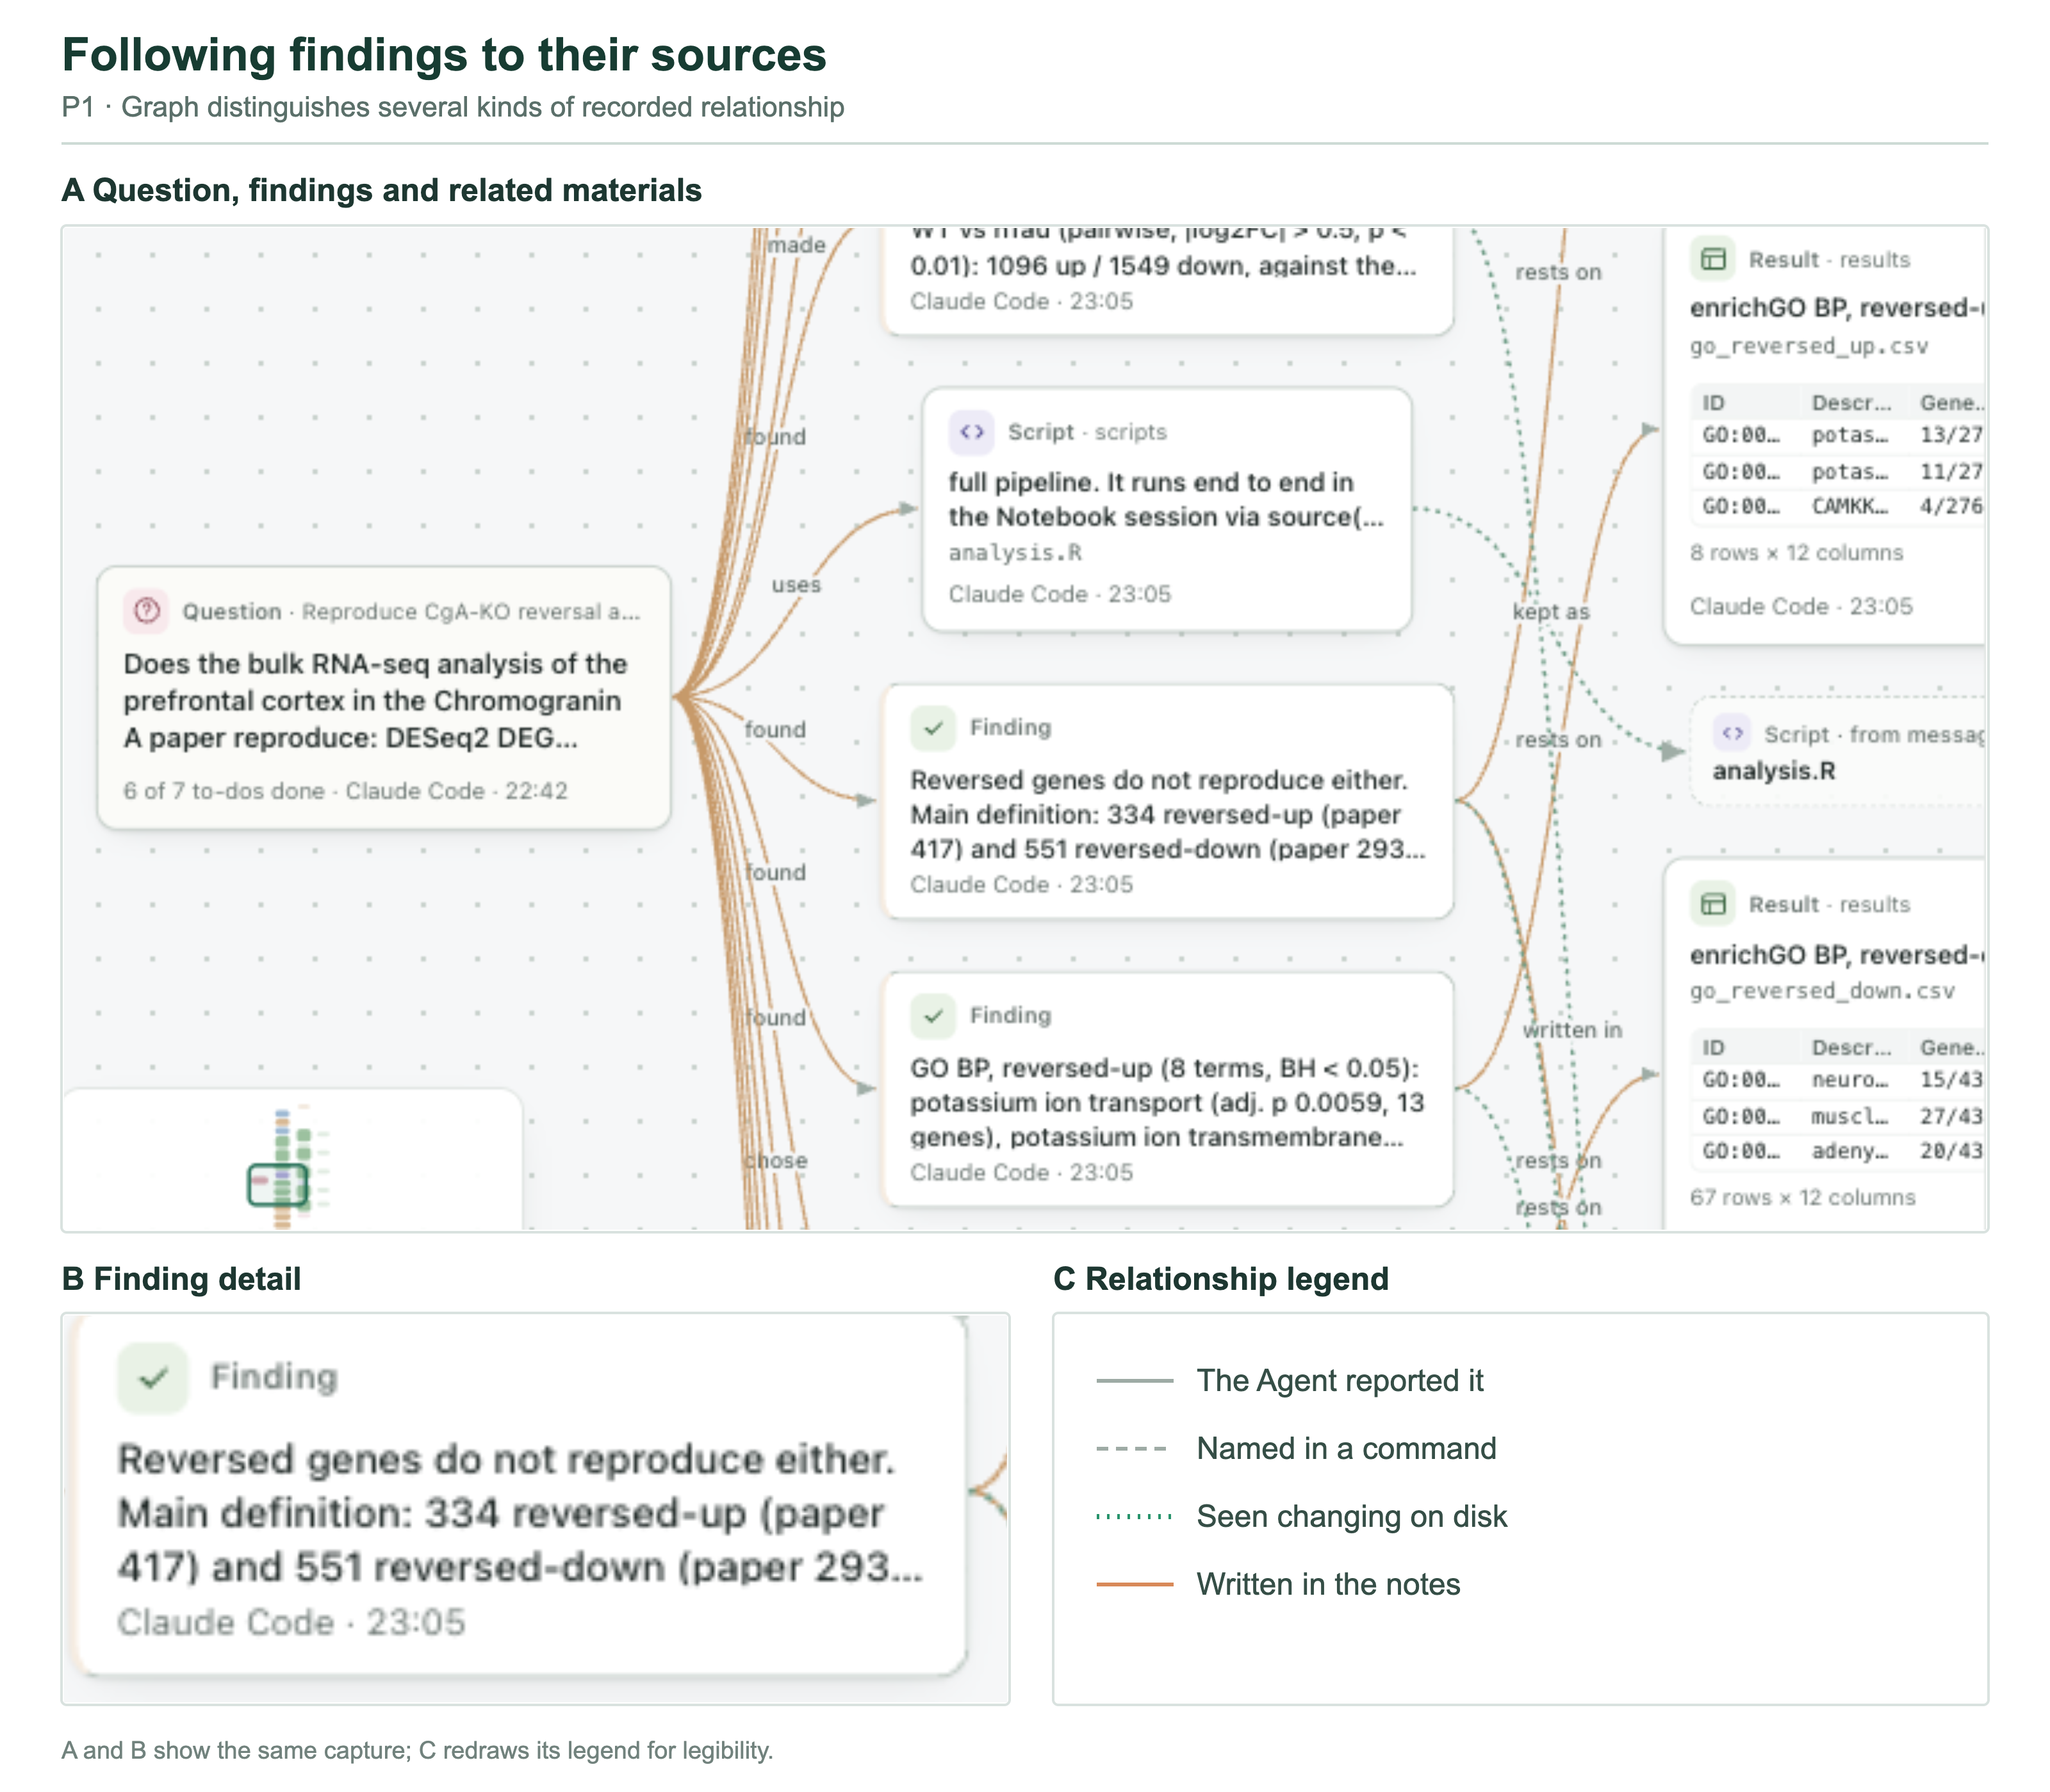
\includegraphics[width=\linewidth,height=0.9\textheight,keepaspectratio]{figures/figure-3-graph.png}
\caption{\textbf{Figure S3. P1 in Graph.} (A) A graph region relating a question, findings, script and result files; (B) an enlarged finding detail; (C) the relationship legend, redrawn for legibility. Edges make recorded associations navigable; they do not certify a scientific explanation.}\end{figure}

\begin{figure}[!htbp]\centering
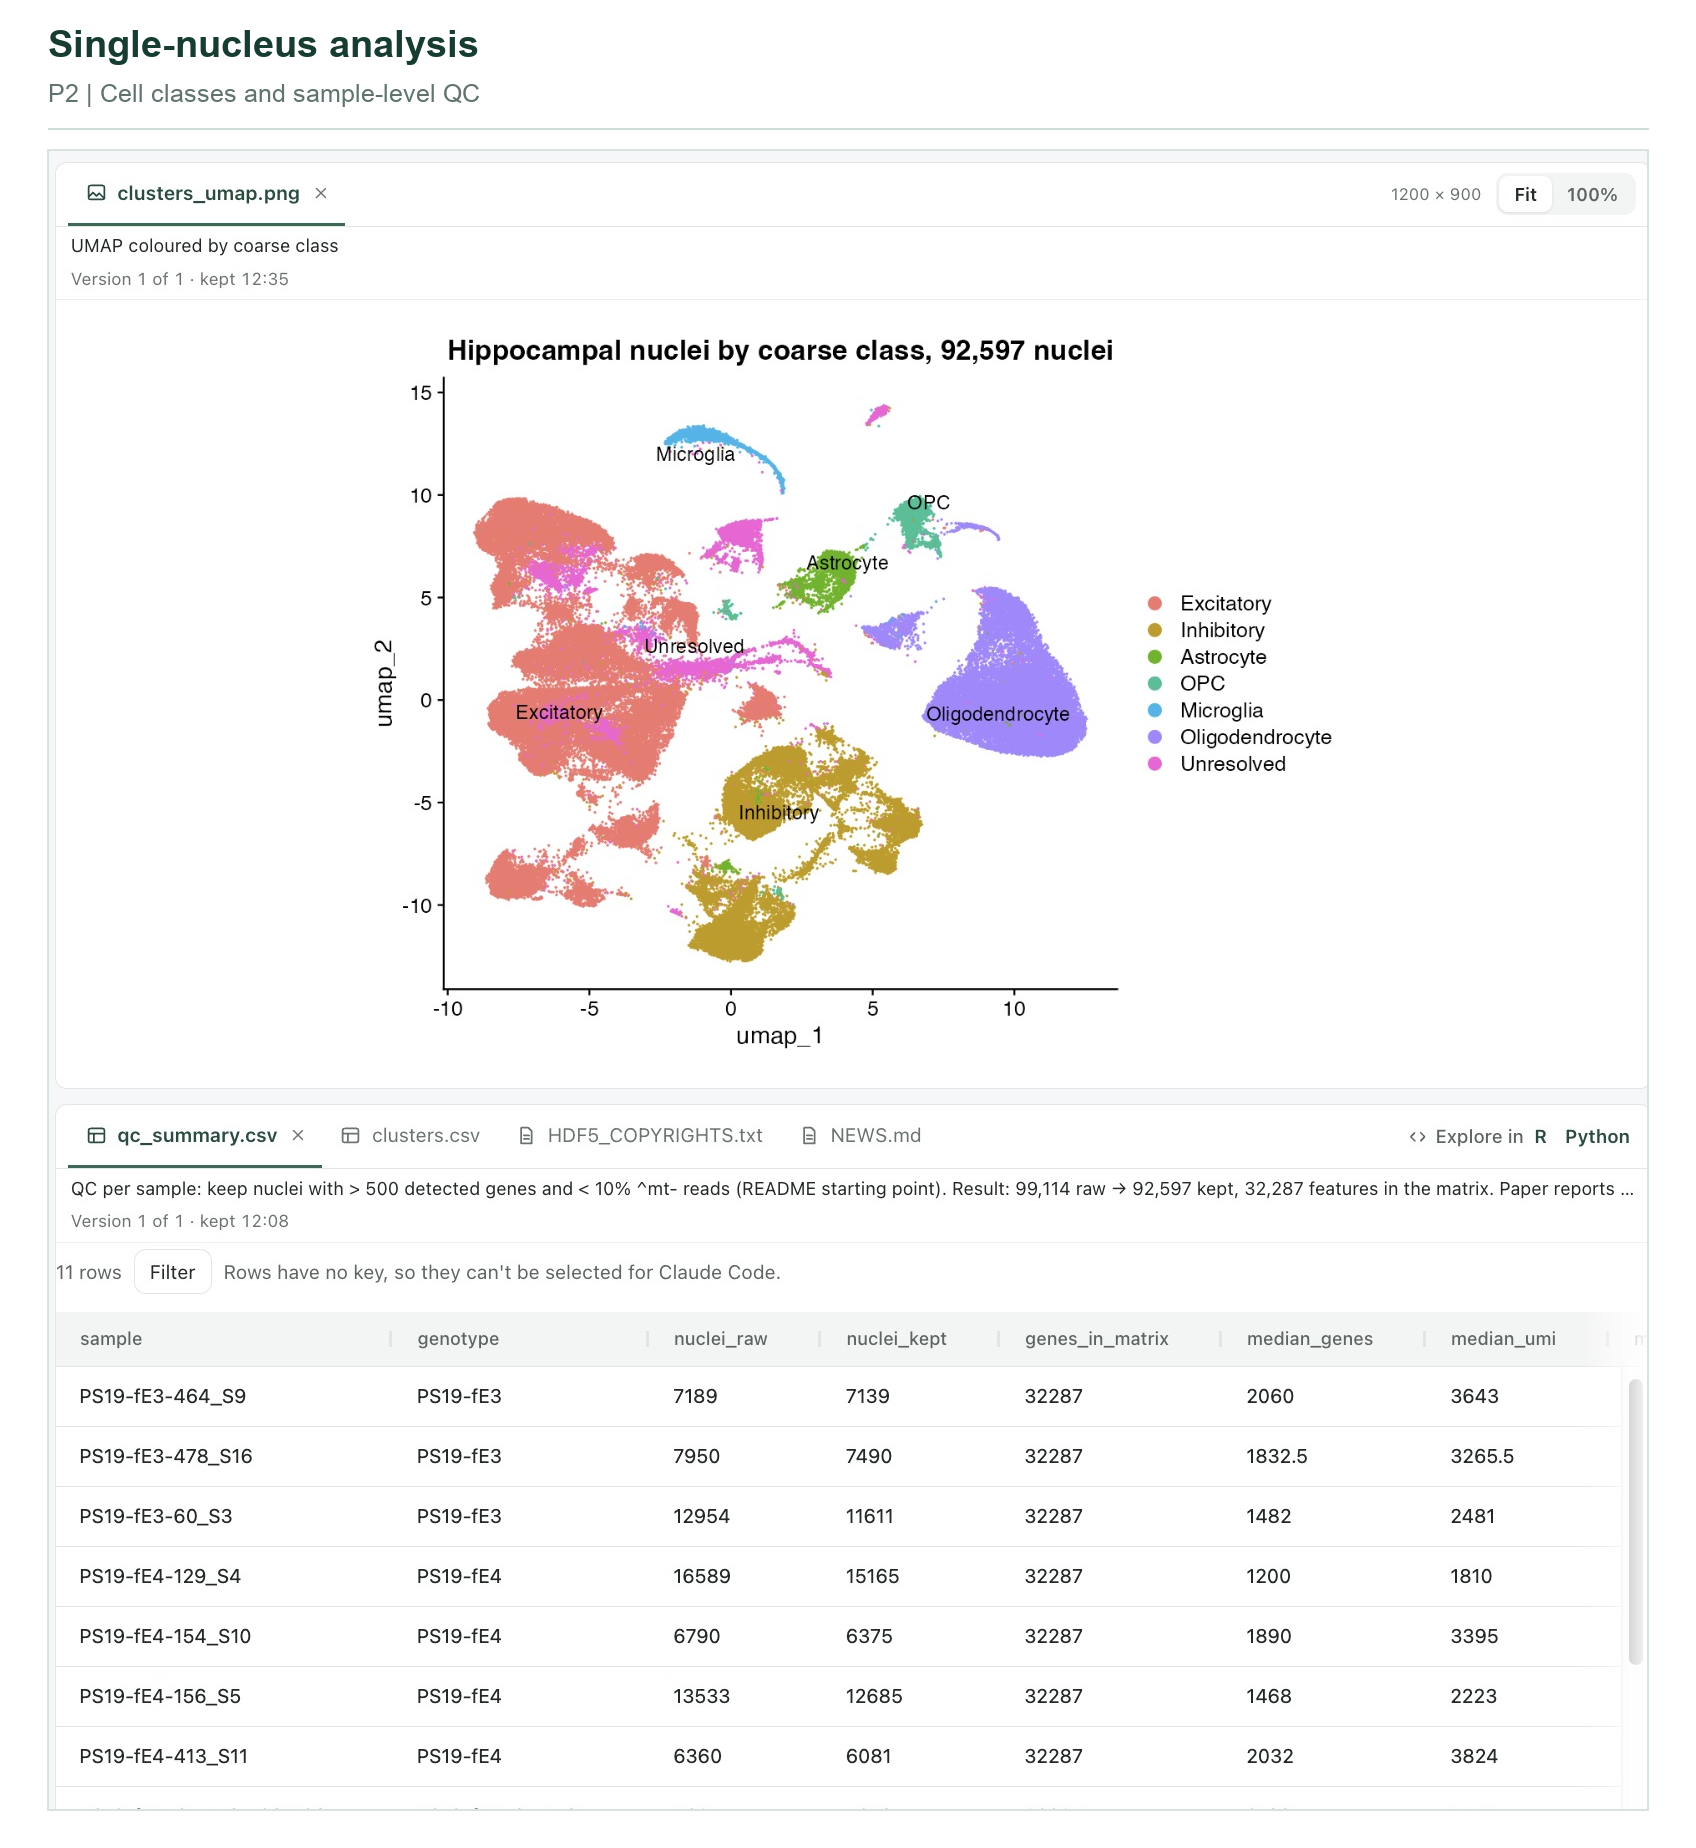
\includegraphics[width=\linewidth,height=0.9\textheight,keepaspectratio]{figures/figure-4-p2.png}
\caption{\textbf{Figure S4. P2 in Studio.} The saved UMAP and per-sample QC table, reopened after the run (source capture $3840\times1972$). The classes are preliminary and the R session was no longer live at capture.}\end{figure}\FloatBarrier

\begin{figure}[!htbp]\centering
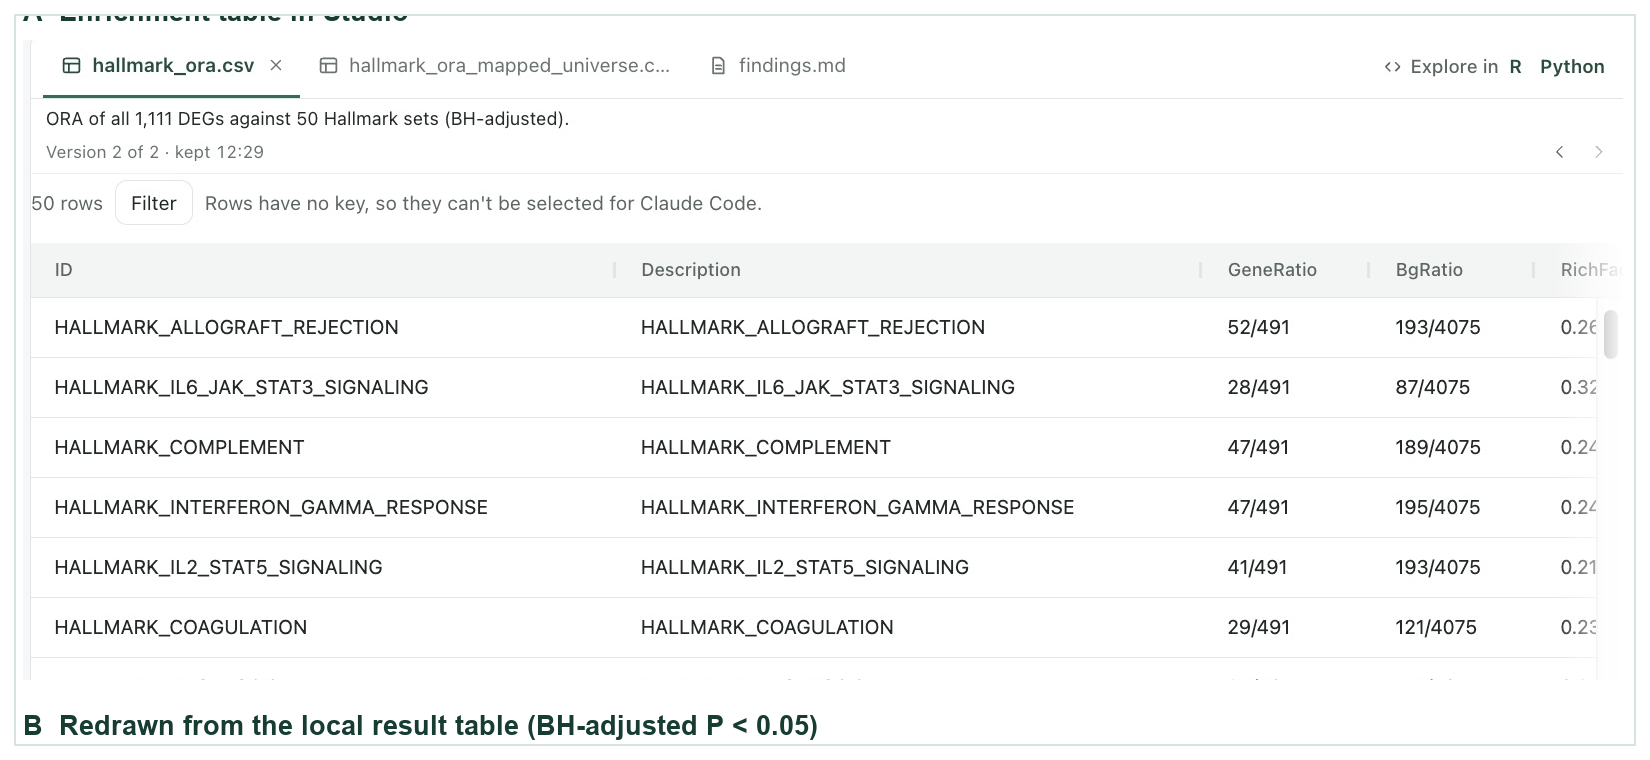
\includegraphics[width=\linewidth,height=0.9\textheight,keepaspectratio]{figures/figure-5-p3-studio.png}
\caption{\textbf{Figure S5. P3 in Studio.} The saved Hallmark over-representation table as it appeared in the reopened project ($3840\times1972$ capture). The 13 significant terms are re-plotted in the main text (Figure~5); the redraw is not a new enrichment analysis.}\end{figure}

\begin{figure}[!htbp]\centering
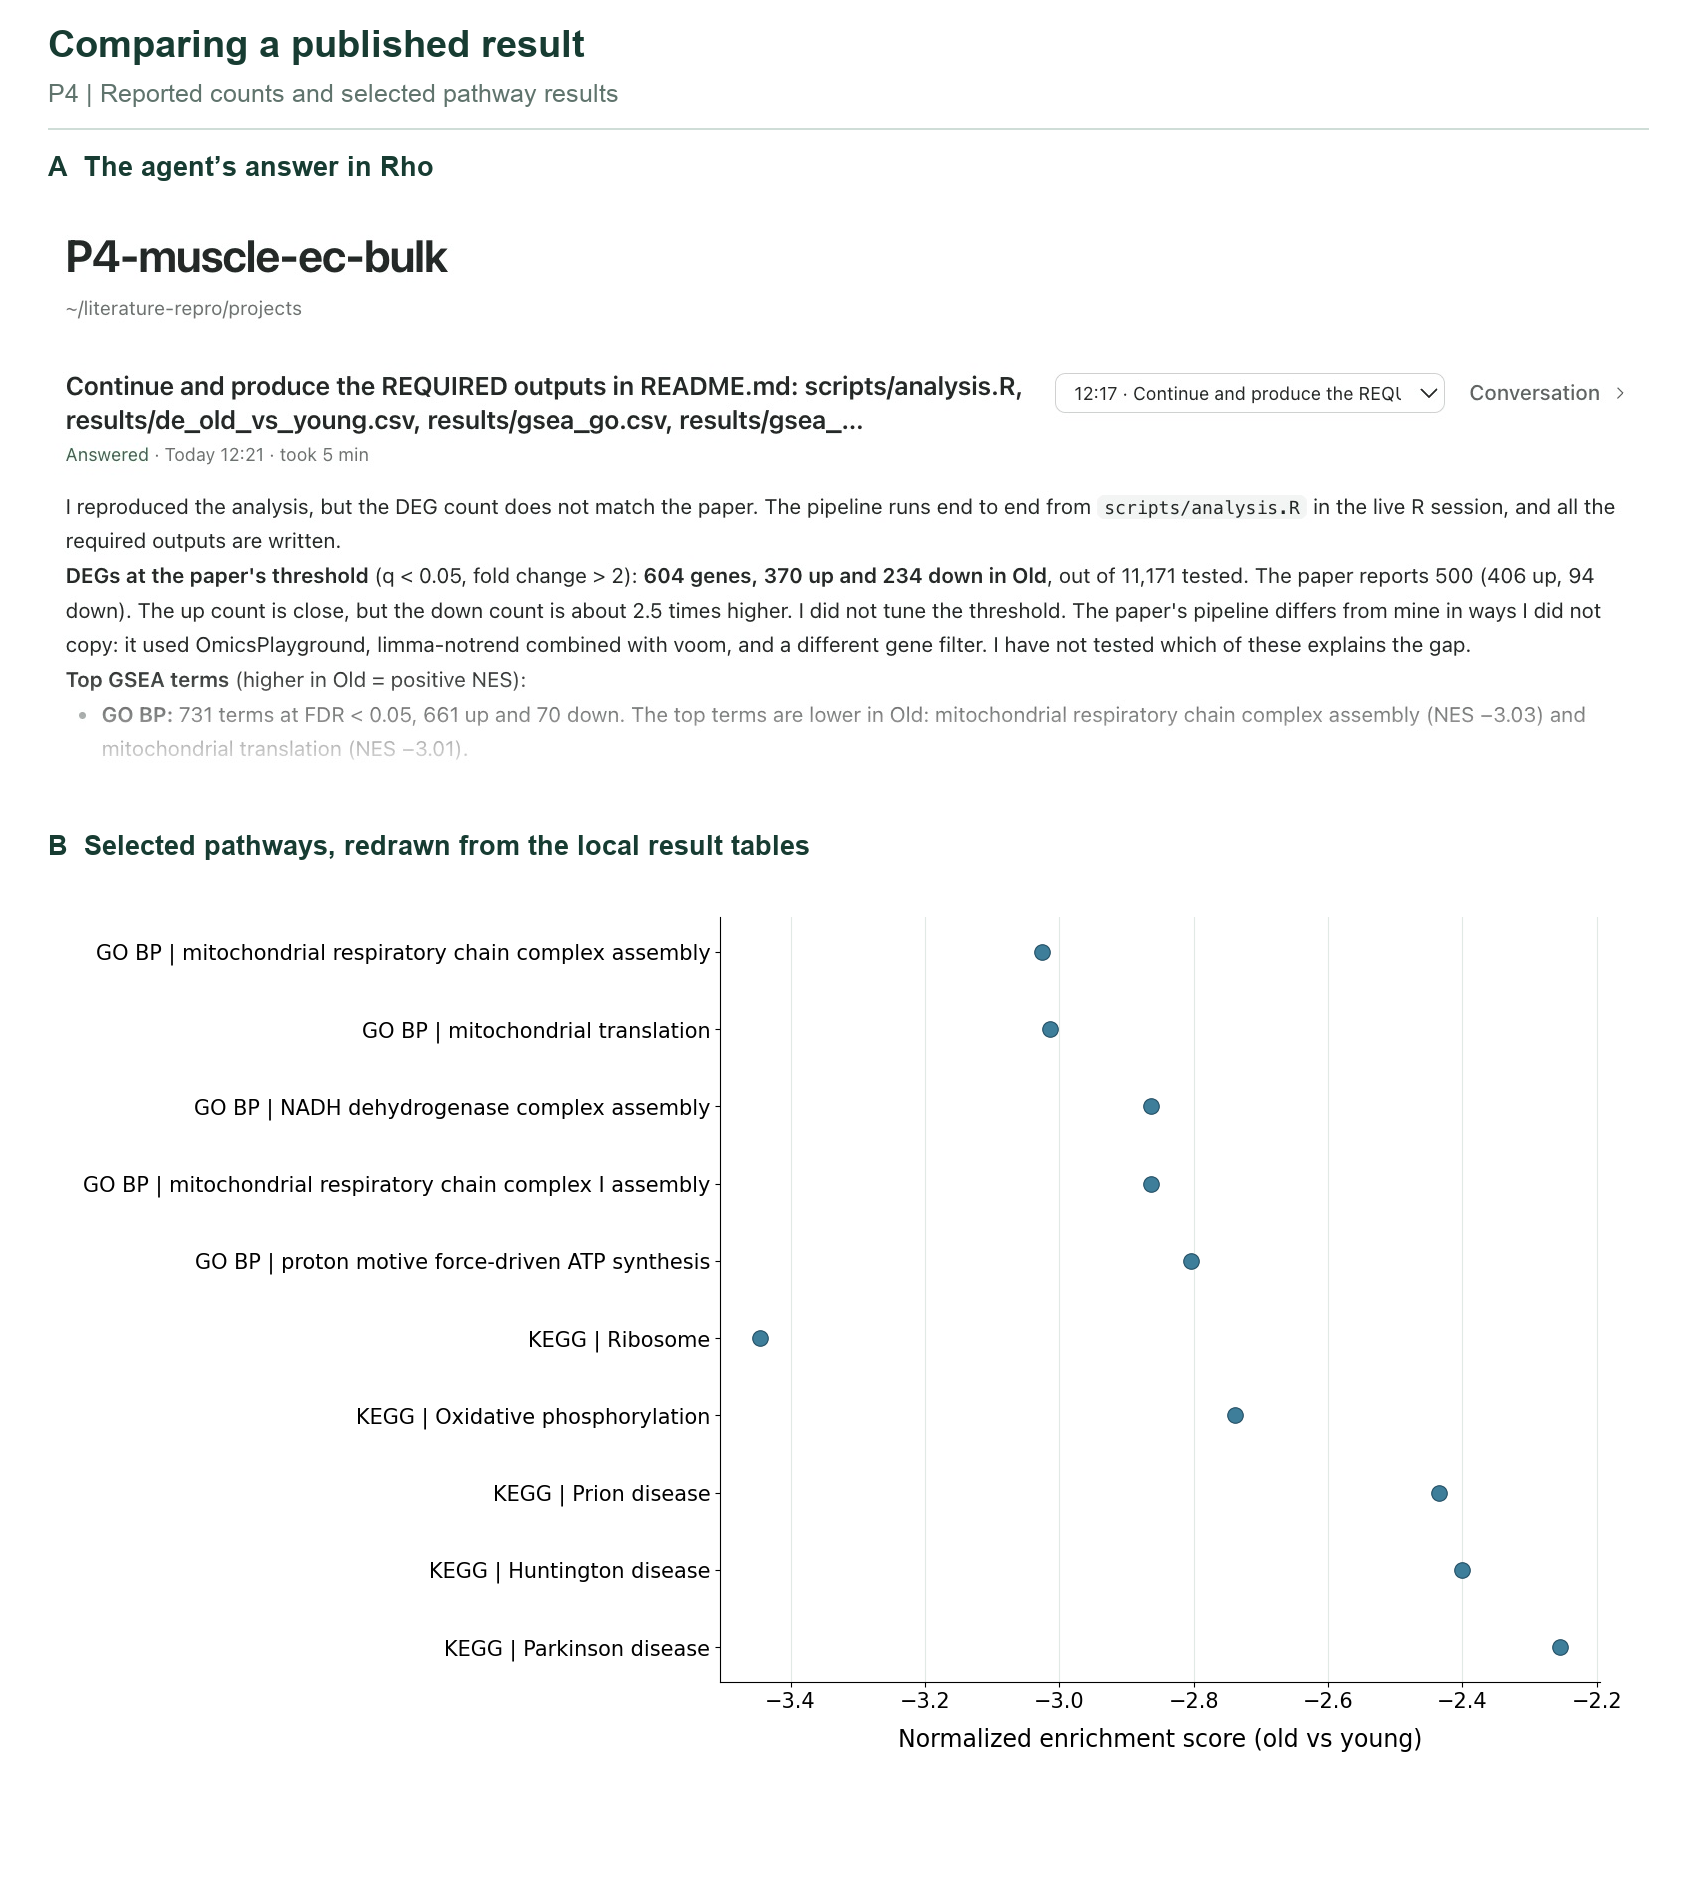
\includegraphics[width=\linewidth,height=0.9\textheight,keepaspectratio]{figures/figure-6-p4.png}
\caption{\textbf{Figure S6. P4 overview and selected pathways.} (A) The agent's reported counts; (B) a redraw of the five lowest-adjusted-P terms from each local GO BP and KEGG table. The answer is the agent's interpretation, not independent validation.}\end{figure}\FloatBarrier

\begin{figure}[!htbp]\centering
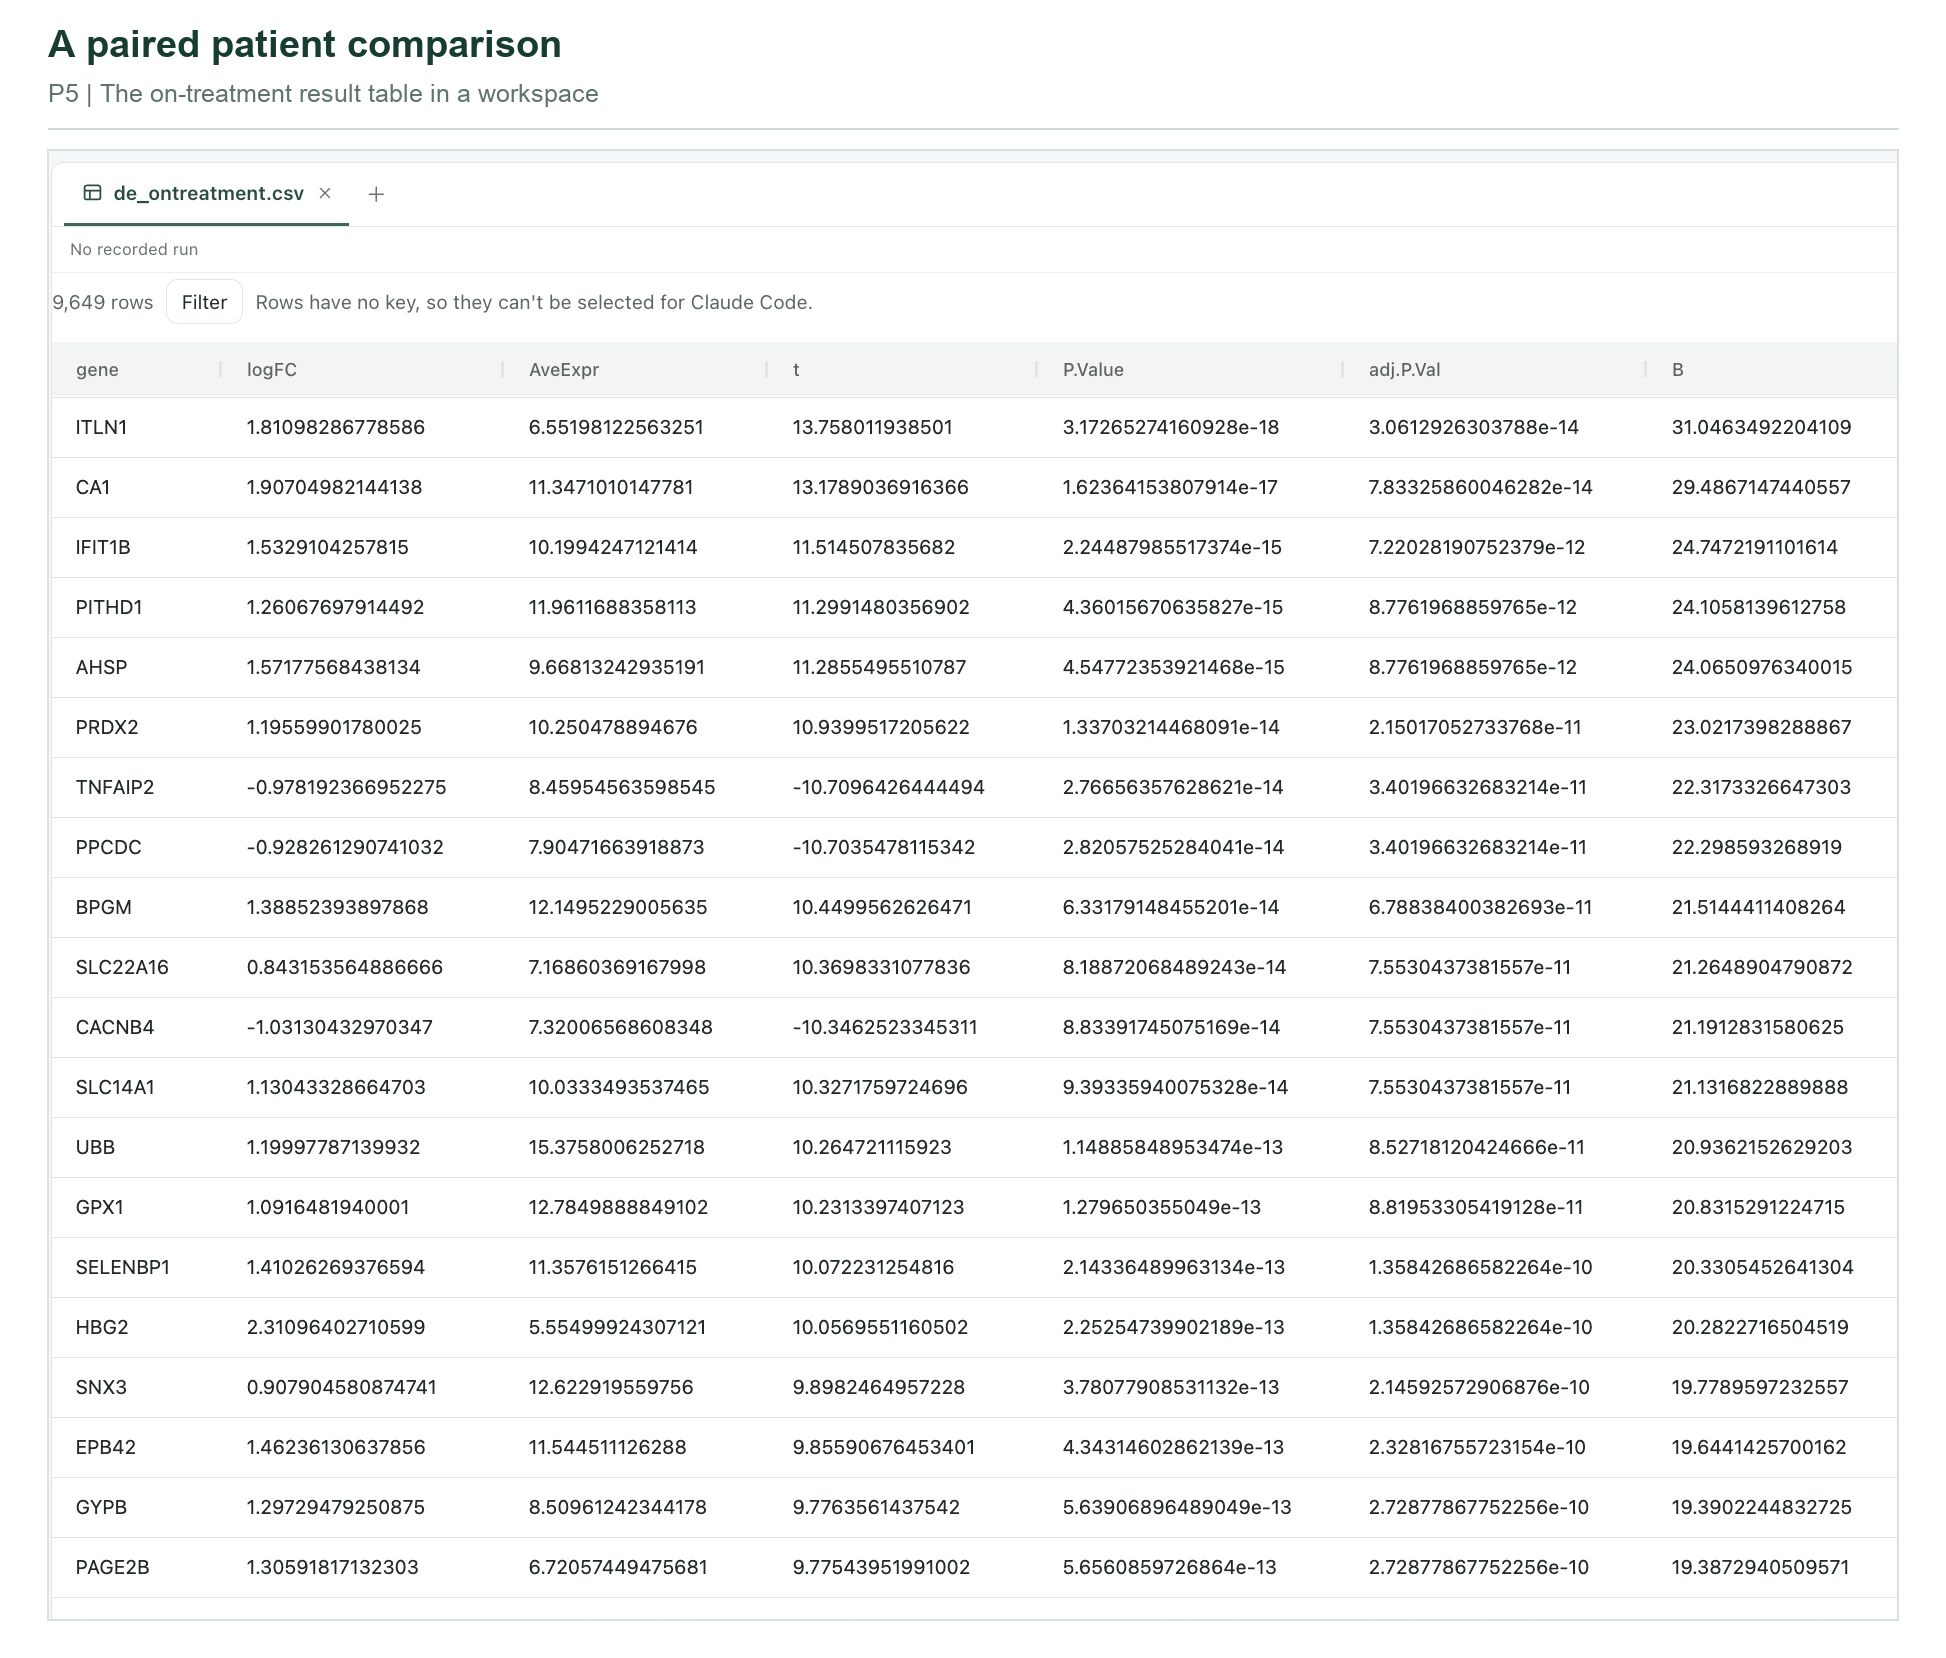
\includegraphics[width=\linewidth,height=0.9\textheight,keepaspectratio]{figures/figure-7-p5.png}
\caption{\textbf{Figure S7. P5 in Studio.} The saved on-treatment versus baseline patient-level table, reopened after the run; the historical notebook and project records are needed to inspect its analysis context.}\end{figure}

\begin{figure}[!htbp]\centering
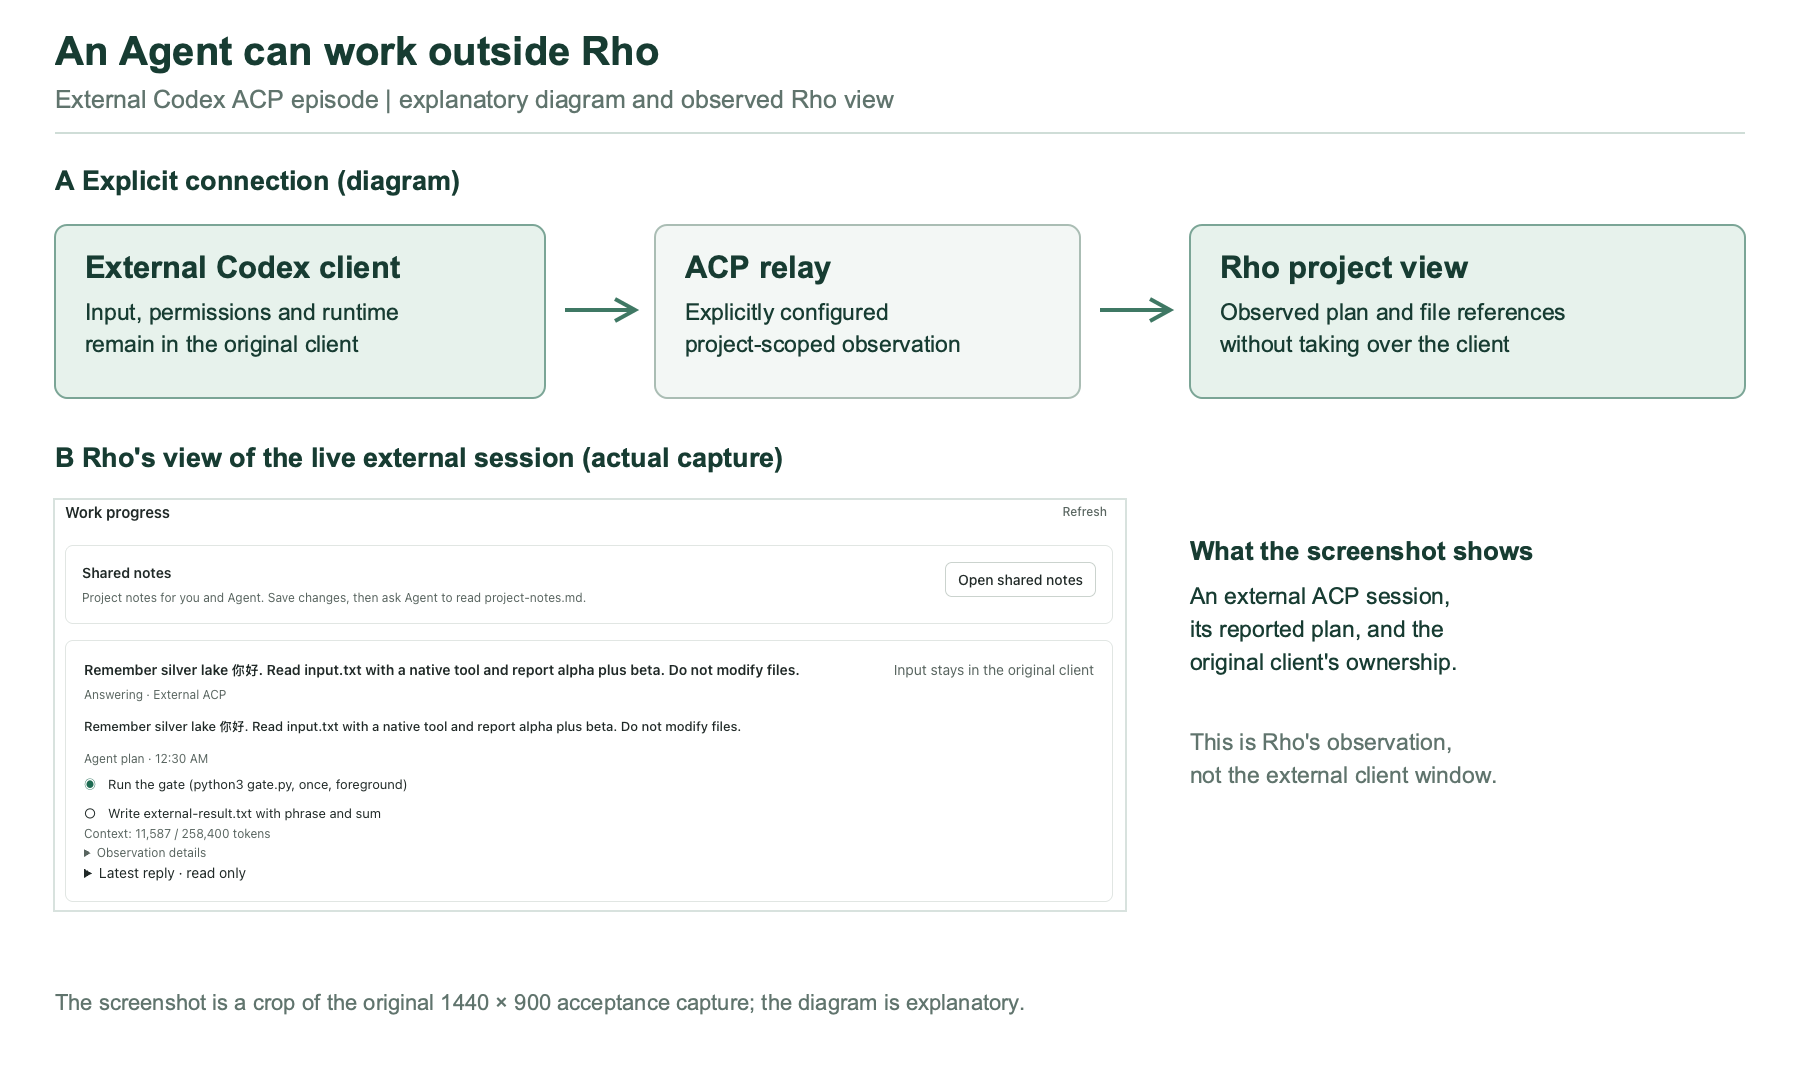
\includegraphics[width=\linewidth,height=0.9\textheight,keepaspectratio]{figures/figure-8-external-agent.png}
\caption{\textbf{Figure S8. An external agent and Rho.} (A) An explanatory diagram of the explicit ACP connection; (B) a Rho-side capture during the separate installed external Codex episode, showing a live reported plan (original $1440\times900$); it does not show the external client window. This episode used a different package composition from the five 0.5.2 analysis projects.}\end{figure}

\end{document}
